%| Weekly report template for CSUS Senior Design
%|
%| language: LaTeX
%| Author: Ben Smith
%| 
%| This source has been tagged with the "<CHANGE" tag in areas
%| that require updating when making a new docuent
%|
%| This source will generate a PDF file complete with thumbnails navigation menu and metadata.
%| Much of the tex awesomeness comes from http://www.michaelshell.org/ praise be to him for creating the guide
\documentclass[11pt,journal]{IEEEtran}

%| Override compsoc class' Palatino font for body text, restores to Times New Roman
\renewcommand{\rmdefault}{ptm}\selectfont

%| IEEE Citation package
 \usepackage{cite}

%| American Mathematical Society package for fancy maths	
\usepackage[cmex10]{amsmath}
\interdisplaylinepenalty=2500				% Restores IEEE line spacing after amsmath

\usepackage{fixltx2e}

\usepackage{graphicx}

\usepackage{float}

\usepackage{wrapfig}

%| Improved URL handling
\usepackage{url}

\usepackage{float}

%| Enables PDF metadata, thumbnails, and navigation
\newcommand\MYhyperrefoptions{
	bookmarks=true,
	bookmarksnumbered=true,
	pdfpagemode={UseOutlines},
	plainpages=false,
	pdfpagelabels=true,
	colorlinks=true,
	linkcolor={black},
	citecolor={black},
	pagecolor={black},
	urlcolor={black},
	pdftitle={Lab One: Signals And Measurements},							
	pdfsubject={EEE108},													
	pdfauthor={Benjamin Smith},	
	pdfkeywords={Weekly Report}}					

%| Calls hyper ref package 
\usepackage[\MYhyperrefoptions,pdftex]{hyperref}

% correct bad hyphenation here
\hyphenation{op-tical net-works semi-conduc-tor}

\renewcommand{\topfraction}{0.9}	% max fraction of floats at top
\renewcommand{\bottomfraction}{0.8}	% max fraction of floats at bottom
%   Parameters for TEXT pages (not float pages):
\setcounter{topnumber}{2}
\setcounter{bottomnumber}{2}
\setcounter{totalnumber}{4}     % 2 may work better
\setcounter{dbltopnumber}{2}    % for 2-column pages
\renewcommand{\dbltopfraction}{0.9}	% fit big float above 2-col. text
\renewcommand{\textfraction}{0.07}	% allow minimal text w. figs
%   Parameters for FLOAT pages (not text pages):
\renewcommand{\floatpagefraction}{0.7}	% require fuller float pages
% N.B.: floatpagefraction MUST be less than topfraction !!
\renewcommand{\dblfloatpagefraction}{0.7}	% require fuller float pages

\begin{document}

%| =================================================================================================
%| Title Block
%| =================================================================================================
\title{EEE108L: Electronics Laboratory \\
	Lab One: Basic Signals and Measurements}
\author{Ben Smith - \today}
\date{\today}
\maketitle

%| =================================================================================================
%| Weekly time report
%| =================================================================================================
\section{Introducton}
	\IEEEPARstart{T}{his} lab is an exercise in measurement and equipment usage. The first section investigates 
	the signal generator and it's non-ideal characteristics that impact voltage measurements. The second section introduces the student
	to a number of advanced techniques with the oscilloscope. Part two uses the Oscilloscope to identify the forward bias on a diode.

\section{Part one: The Function Generator and Oscilloscope}
	
	\IEEEPARstart{I}{n} this section the effect of the signal generator's output impedance on measurements is analyzed. The section "Output Termination"	
	of the Agilent 33120A user manual provides insight into the generator's settings. The voltage displayed is not a measurement of the
	output it is a stored value for the output setting. The display is an approximation of the output voltage based on a 50$\Omega$ terminated circuit.
	\begin{wrapfigure}[12]{l}{.26\textwidth}
		\centering
		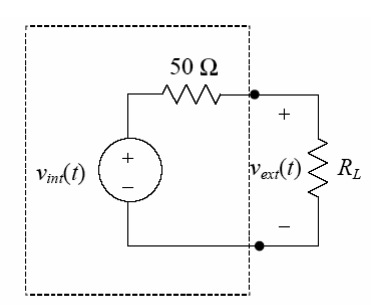
\includegraphics[width=.25\textwidth]{screenshot_22}
		\caption{Thévenin internal view of generator\cite{2}} 
	\end{wrapfigure}
	
	The 50$\Omega$ termination setting is designed for representing voltage delivered to terminated loads accurately. The setting halves the voltage output 
	with respect to what is on the display. Figure 1 shows the elements that contribute to this phenomenon diagrammatically. This system can be modeled using 
	a resistive divider, as seen line 1 below. 
	
	\begin{eqnarray}
		V_{out} &=& V_{in} \frac{R_2}{R_1 + R_2}\\
		V_{ext} &=& V_{out}(t)\frac{R_L}{R_L + 50\Omega}
	\end{eqnarray}
	Equation 3 shows the result of the resistive divider that a infinite value (hi-z) of $R_L$ will drive the resistive dependent term to one.

	\begin{eqnarray}
		\lim_{R_L \rightarrow \infty} V_{out}(t)\frac{R_L}{R_L + 50\Omega} &=& V_{out}(t)
	\end{eqnarray}
	
	Equation 4 shows the other case, if set $R_L$ to 50$\Omega$ $V_{out}$ is halved. 
	
	\begin{eqnarray}
		V_{out}(t) \frac{50\Omega}{50\Omega + 50\Omega} &=& \frac{V_{out}(t)}{2}
	\end{eqnarray}
	
		\subsection{Step One}
		
			Equation 2 is tested in the experimental environment. Table one lists the 
		experimental data and their discrepancies can be explained by the function generator's
		terminations settings at $50\Omega$
		
		\begin{table}[htpb]
			\renewcommand{\arraystretch}{1.2}
			\caption{Labratory Data}
			
			\label{Team Hour Summary}
			\centering
			\begin{tabular}{r|p{1.7cm}|p{1.8cm}| p{1.5cm}}
			\hline
			\bfseries 	Parameter	 					&  \bf Oscilloscope Measurement			& \bfseries Function Generator Display 		& \bfseries Scope with 100 $\Omega$ load	\\
			\hline\hline
						Amplitude,  $V_{PP}$			& 3.04									& 1.4										& 2.08		\\
						Frequency, $Hz$					& 600									& 599.1										& 600.6		\\	
						Offset, $V$						& -0.5									& -0.550									& -0.317	\\
			\hline
			\end{tabular}
		\end{table}
	
		The doubling of the oscilloscope measurement from the function generator display is expected. The $0.4V$ volt discrepancy
		can be attributed to the non ideal load of the oscilloscope.
	
	\subsection{Step Two: Load the signal generator's output}
		When the signal generator's output was loaded the reading on it's display did not change. This would be expected as the
		display is a setting for an internal control system, not a measurement of the output. The voltage on the display also removes 
		DC offset from the input signal. This can be useful when measuring signals that are transmitted across a real medium with 
		inherit capacitance.
		
	\subsection{Step Three: Coupling}
		Changing the coupling on the oscilloscope centers an AC waveform about the vertical axis. The AC coupling mode provides a convenient way to view
		a signal without DC offset.
			
	\subsection{Step 4: The trigger signal}
		The trigger signal changes states based on the output wave. For sine ramp and pulse waveforms the sync signal is
		logic high when the output voltage is above the average value of the signal, low when it's below \cite{3}. The signal generator user's guide discusses
		the different operating modes for the sync signal. When the signal's amplitude, and offset parameters are adjusted the sync signal did not change.
		When the frequency setting is changed the sync signal changes frequency to stay in step with the output waveform. Figure two illustrates the two waveforms at 500Hz.
	
	\begin{figure}[H]
		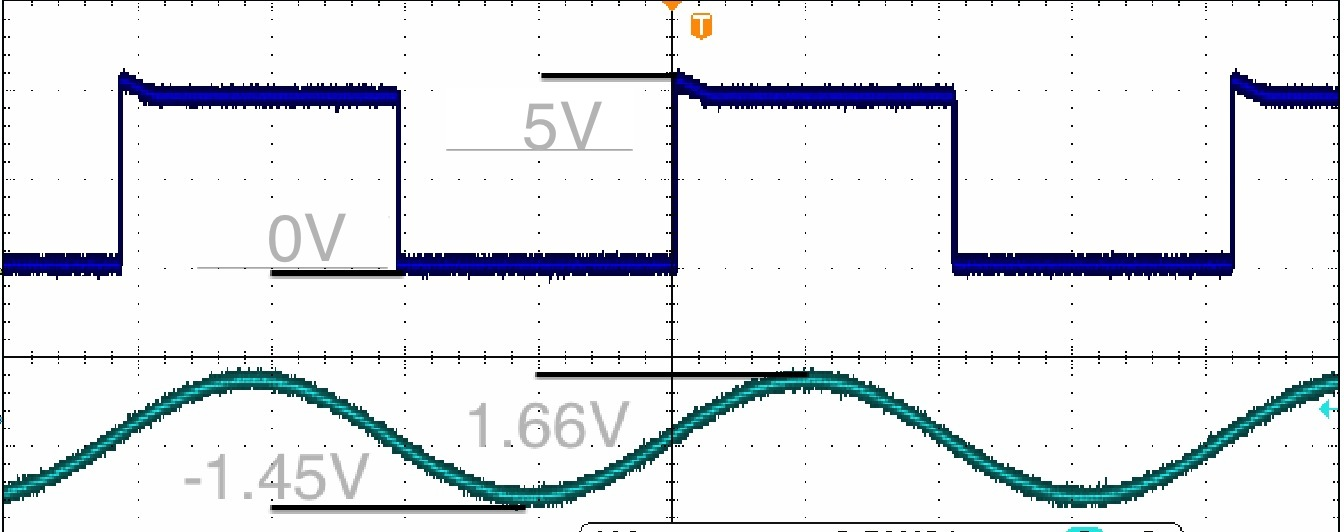
\includegraphics[width=.5\textwidth]{screenshot_25}
		\caption{Function generator output sync and output signals}
	\end{figure}
	
	\subsection{Step 6: Oscilloscope trigger parameter}
		The sinusoidal input changes amplitude with respect to time. The trigger aligns the signal crossing with the vertical axis, this alignment causes a false horizontal shift to appear.
	
	\subsection{Step 7: Trigger threshold adjustment with square wave}
		The square wave had a very fast rise time compared to the frequency of the signal. There was no observable movement along the time axis while the
		trigger was set between the high and low states of the signal.
	
	\section{Part Two: A Simple Diode Circuit}	
		\begin{wrapfigure}[12]{l}{.26\textwidth}
			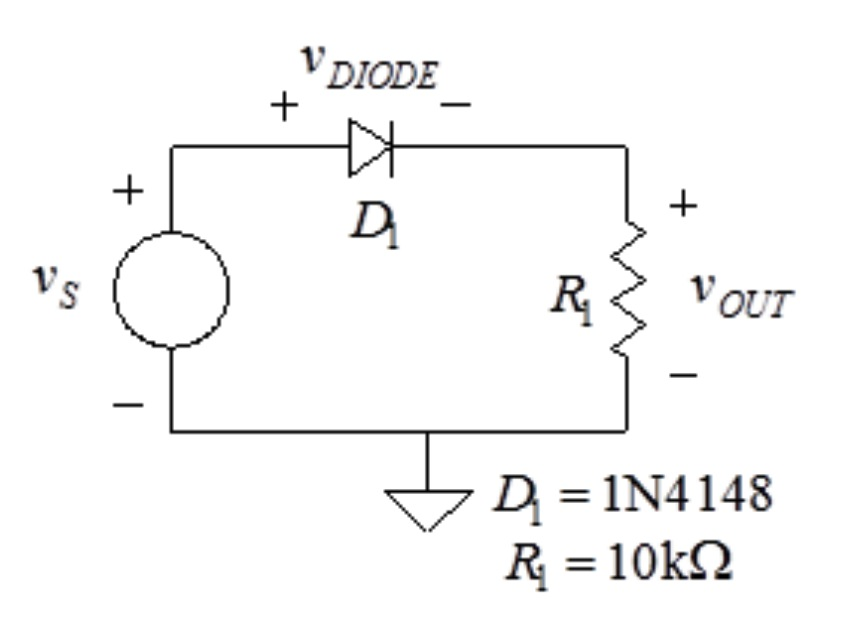
\includegraphics[width=.25\textwidth]{screenshot_27}
			\caption{Circuit specification in lab manual}
		\end{wrapfigure}
		A single loop diode circuit was assembled as depicted in figure 3. When a alternating current signal was placed across $D_1$ the signal is rectified. The output signal of the system
		shows it is behaving as a half wave rectifier.
		
		The dark blue wave in Figure 4 is the input of the system $V_s$. The light blue signal is $V_{out}$. Figure 4 shows Diode $D_1$ experiences maximum forward bias when the input signal is at it's lowest value.
			
	\begin{figure}
		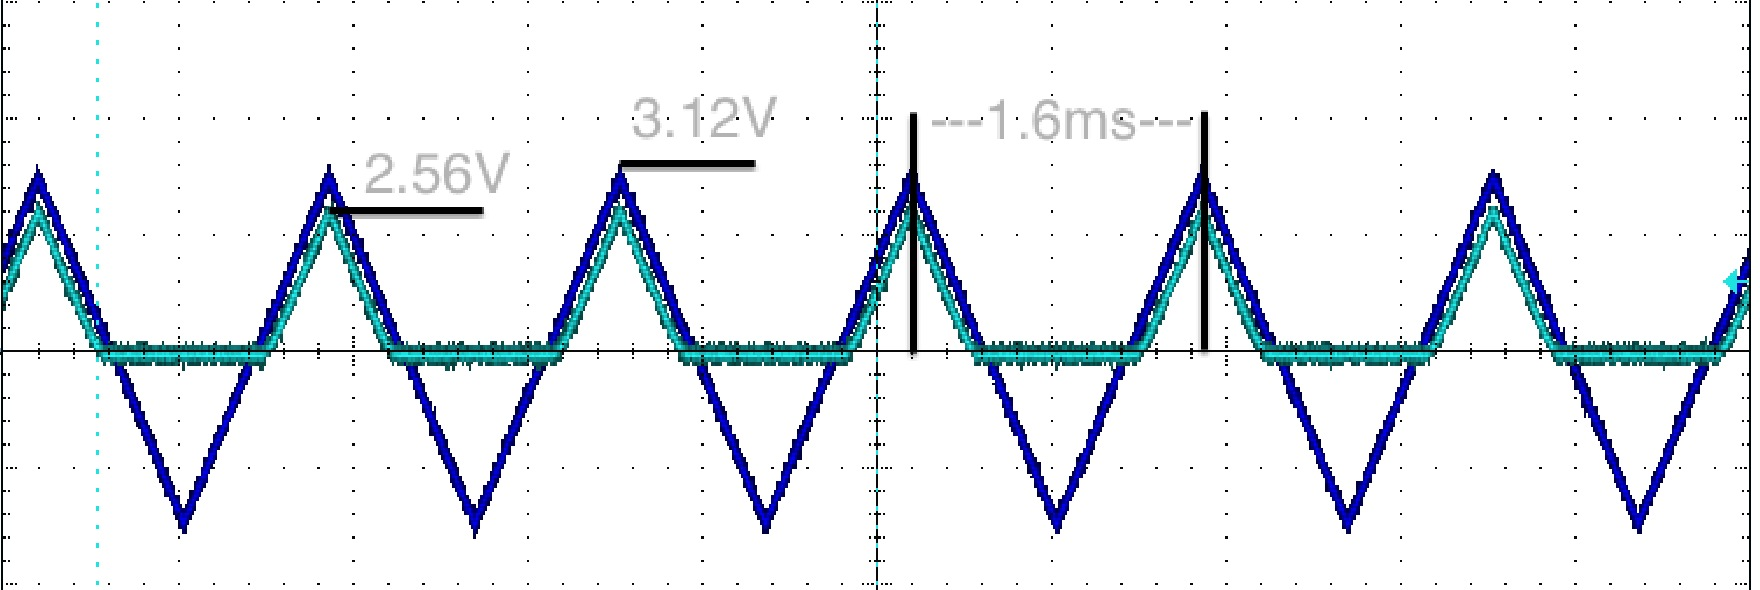
\includegraphics[width=.5\textwidth]{screenshot_26}
		\caption{Rectified triangle wave}
	\end{figure}
	
	The red wave in figure 5 is the difference between input and output voltage on a scale that's half the blue waveforms $(\frac{1V}{div})$. The red waveform is the amount of forward bias on the diode. The troughs of the blue and red
	waveforms align showing relationship expected. 
	
	\begin{figure}
		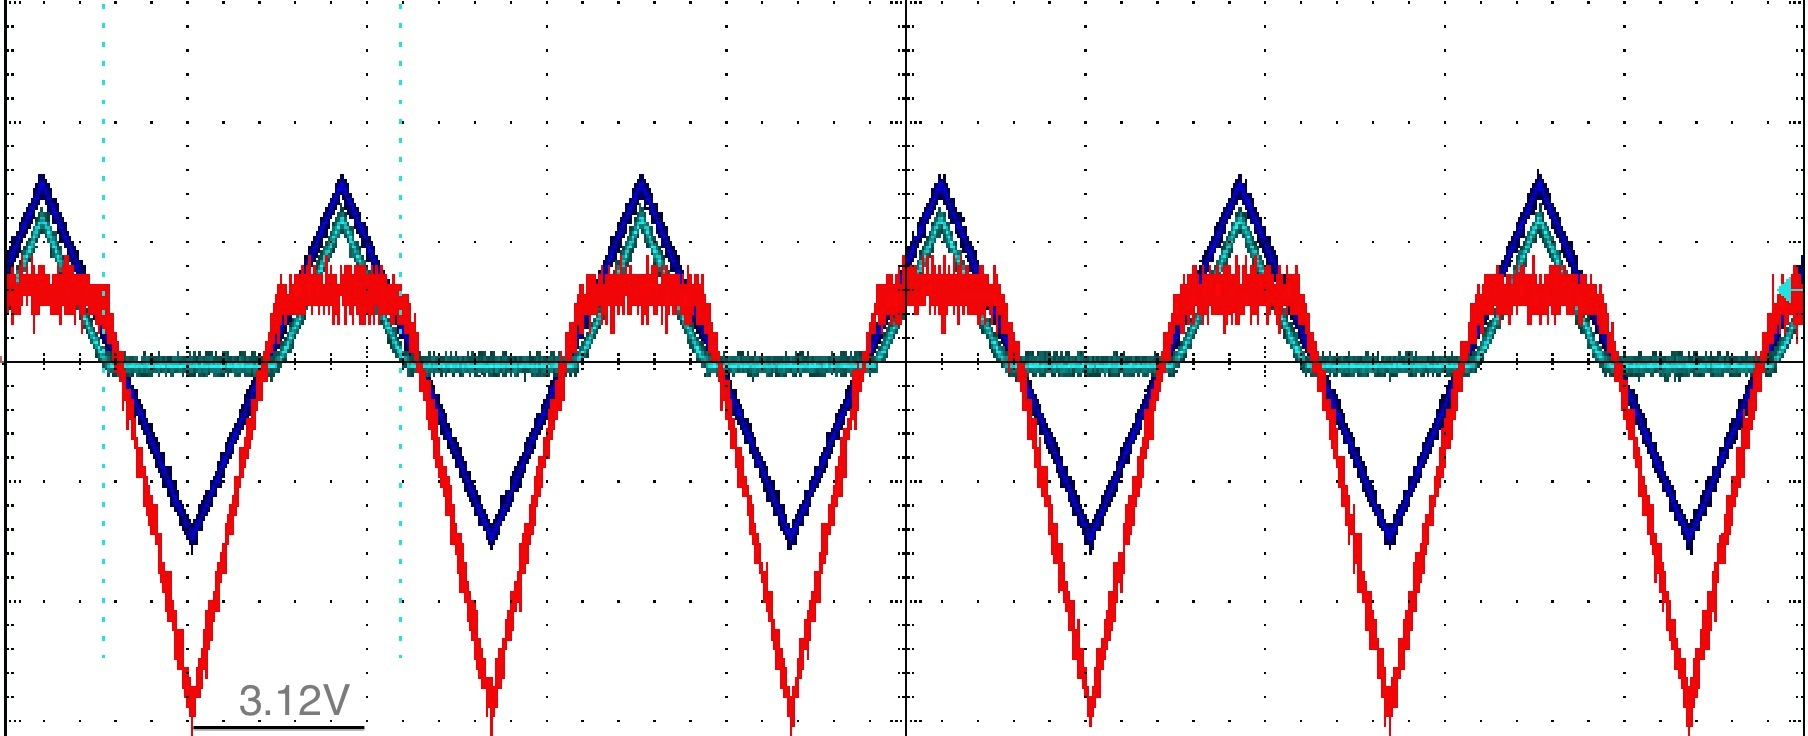
\includegraphics[width=.5\textwidth]{screenshot_28}
		\caption{Rectified triangle wave with difference superimposed}
	\end{figure}
	
	\section{Conclusions}
		\subsection{Item 1}
		The output voltage of the function generator varies in accordance with Equation 3. Figure 6 is Equation 3 with $V_{out}(t)$ is assumed to be a constant one and $R_L$
		is the independent variable.
		
		\begin{figure}[H]
			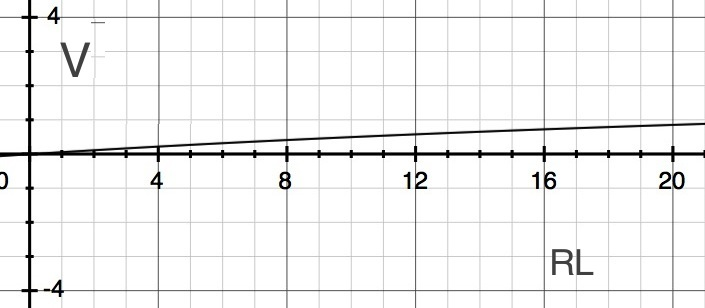
\includegraphics[width=.5\textwidth]{screenshot_30}
			\caption{Unit output voltage as a function of $R_L$}
		\end{figure}
		Figure 6 shows a narrow window to emphasize the change in voltage with respect to the load resistance. The output voltage of the signal generator does change and will only be accurate for 50$\Omega$ terminated loads.
		
		\subsection{Item 2}
		The amplitude on the front panel of the function generator does not change when the signal is loaded by the $100 \Omega$ resistor. The amplitude displayed is not a voltage measurement of the output, it is a pre stored
		calibrated value. The value listed on the function generator is a peak to peak voltage for a 50$\Omega$ terminated signal.
		
		\subsection{Item 3}
		The sync output is always 50\% duty cycle this prevents charge from building on the input line and rising above the trigger voltage. It also allows an oscilloscope to synchronize on a fixed point in
		a generated signal's period. 
		 
		\subsection{Item 4}
		The peak current through diode $D_1$ can be calculated by using the output voltage measured with the oscilloscope.
		
		\begin{eqnarray*}
			I &=& \frac{V}{R}\\ \\
			I &=& \frac{3.12V}{10K\Omega}\\ \\
			I &=& 3.12mA
		\end{eqnarray*}
		
		\subsection{Item 5}
		Modeling the function generator as having an output resistance of zero is acceptable in cases when the resistance of the load is
		much larger then than the generator's source impedance. 
		
		
	%Declare bibliography style
	\bibliographystyle{IEEEtran}
	\bibliography{IEEEfull}

\end{document}